\documentclass[aspectratio=169,pdf,t]{beamer}
\usepackage{defense}


\title{Carbonitruration des alliages 16NiCrMo13 et 23MnCrMo5}
\subtitle{modélisation et procédés}
\author{Walter DAL'MAZ SILVA\inst{1,2}\\[8pt]
  \and {\small Directeur de thèse: Thierry BELMONTE\inst{2}}\\[8pt]
  \and {\small Co-directeur de thèse: Jacky DULCY\inst{2}}}
\institute{
  \inst{1} Institut de Recherche Technologique M2P, Metz, France \and 
  \inst{2} Institut Jean Lamour, Nancy, France}
\date{22 juin 2017}


\begin{document}


\begin{frame}{Composition du jury}
  \vfill%
  \begin{tabular}{p{0.22\textwidth}p{0.50\textwidth}p{0.28\textwidth}}
  	M. M. Gouné
  	& Professeur, Université de Bordeaux
  	& Rapporteur 
  	\tabularnewline[5pt]
  	M. C. Vahlas
  	& Directeur de recherche, CIRIMAT, Toulouse
  	& Rapporteur 
  	\tabularnewline[5pt]  
  	Mme. M.-L. Giorgi
  	& Professeur, LGMP, Châtenay-Malabry
  	& Examinateur 
  	\tabularnewline[5pt]  
  	M. F. Mudry
  	& Président, IRT M2P, Metz
  	& Examinateur 
  	\tabularnewline[5pt]   
  	Mme. I. Ziegler-Devin
  	& Maître de conférences, LERMAB, Nancy
  	& Examinateur 
  	\tabularnewline[5pt]  
  	M. S. Thibault
  	& Docteur-ingénieur, Safran Tech, Magny-les-Hameaux
  	& Examinateur 
  	\tabularnewline[5pt]
  	M. J. Dulcy
  	& Ingénieur de recherche, IJL-CP2S, Nancy
  	& Examinateur
  	\tabularnewline[5pt]  
  	M. T. Belmonte
  	& Directeur de recherche, IJL-CP2S, Nancy
  	& Directeur de thèse 
  	\tabularnewline[5pt]
  \end{tabular}
  \vfill%
  \includegraphics[width=3cm]{figures/logo/ul}
  \hfill%
  \includegraphics[width=2cm]{figures/logo/emma}
  \vfill%
\end{frame}


\begin{frame}{Partenaires TTA}
	\centering{}
	\vspace{-0.5cm}
	
	\def\radius{3.4}
	
	\resizebox{9cm}{!}{
		\begin{tikzpicture}
		\node at (0:0)            {\includegraphics[scale=0.15]{figures/logo/irt.jpeg}};
		\node at (0:\radius)      {\includegraphics[scale=0.25]{figures/logo/ijl.png}};
		\node at (32.72:\radius)  {\includegraphics[scale=0.06]{figures/logo/acelor.png}};
		\node at (59.00:\radius)  {\includegraphics[scale=0.25]{figures/logo/airbus.jpg}};
		\node at (98.18:\radius)  {\includegraphics[scale=0.15]{figures/logo/airliquide.jpg}};
		\node at (132.91:\radius) {\includegraphics[scale=0.12]{figures/logo/ascometal.jpg}};
		\node at (157.64:\radius) {\includegraphics[scale=0.25]{figures/logo/ecm.jpg}};
		\node at (186.36:\radius) {\includegraphics[scale=0.18]{figures/logo/faurecia.jpg}};
		\node at (215.09:\radius) {\includegraphics[scale=0.10]{figures/logo/safran.jpg}};
		\node at (248.82:\radius) {\includegraphics[scale=0.13]{figures/logo/psa.png}};
		\node at (300.55:\radius) {\includegraphics[scale=0.30]{figures/logo/poclain.png}};
		\node at (330.27:\radius) {\includegraphics[scale=0.30]{figures/logo/utc.jpg}};   
		\end{tikzpicture}}
\end{frame}


\begin{frame}{Sommaire}
  \tableofcontents%
\end{frame}


\section{Introduction}


\begin{frame}{\insertsection}
  \begin{columns}[T]
    \begin{column}{0.61\textwidth}
      \setbeamercolor{normal text}{fg=gray,bg=}
      \setbeamercolor{alerted text}{fg=black,bg=}
      \usebeamercolor{normal text}
      
      \begin{enumerate}
        \item \alert<1->{Traitements thermochimiques de surface:}
        \begin{itemize}
          \item \alert<1->{modification de la composition d'un matériau à travers des}
          \item \alert<1->{procédés utilisant souvent une activation thermique et}
          \item \alert<1->{un milieu de composition ou d'activité contrôlée.}
        \end{itemize}
        \vspace{0.3cm}
        
        \item \alert<2->{La cémentation, la nitruration et la carbonitruration sont des traitements réalisés par l'introduction de, respectivement:}
        \begin{itemize}
          \item \alert<2->{carbone}
          \item \alert<2->{azote}
          \item \alert<2->{carbone et azote}
        \end{itemize}
        \vspace{0.3cm}
        
        \item \alert<3->{Cette étude comprend ces traitements des nuances 16NiCrMo13 et 23MnCrMo5 réalisés par voie gazeuse en utilisant des atmosphères de type \ch{CO - H2}, basées sur \ch{NH3} ou des hydrocarbures ayant comme source le \ch{C2H2}.}
      \end{enumerate}
    \end{column}
    \begin{column}{0.39\textwidth}
      \centering{}
      Source : Safran Group
      
      \includegraphics[width=4cm]{figures/pignon.jpg}
      
      \vspace{0.6cm}
      \onslide<4->{
        Caractéristiques visées: ténacité à c{\oe}ur et résistance à la fatigue et à l'usure en surface.}
    \end{column}
  \end{columns}
\end{frame}


\begin{frame}{\insertsection}
  \only<1>{
  \begin{center}
    \vspace{-0.0cm}
    \includegraphics[width=11cm]{figures/schema-traitement.pdf}
  \end{center}}
  \only<2>{
  \begin{center}
    \vspace{+0.5cm}
    \includegraphics[width=11cm]{figures/schema-methode.pdf}
  \end{center}}
\end{frame}


\begin{frame}{\insertsection}{Objectives}
  \begin{columns}[T]
    \begin{column}{0.7\textwidth}
    De manière générale, cette thèse vise \`a répondre aux questions suivantes:
    \vspace{0.5cm}
    \setbeamercolor{normal text}{fg=gray,bg=}
    \setbeamercolor{alerted text}{fg=black,bg=}
    \usebeamercolor{normal text}

    \begin{itemize}
      \def\itemskip{\\[20pt]}
      \item \alert<1->{Quel est l'effet induit par l'azote sur les réponses mécaniques et métallurgiques à la carbonitruration des aciers faiblement alliés?}
      \itemskip
      
      \item \alert<1->{Est-ce que l'introduction de l'azote dans les aciers présente des avantages technologiques par rapport aux traitements de cémentation?}
      \itemskip
      
      \item \alert<2->{Comment mettre au point le contrôle de l'enrichissement promu par les procédés à partir de l'acétylène et de l'ammoniac à basse pression?}
      \itemskip
      
      \item \alert<2->{Quels sont les niveaux de décomposition des précurseurs \ch{C2H2} et \ch{NH3} en fonction des paramètres opératoires des réacteurs?}
    \end{itemize}
    \end{column}
    \begin{column}{0.3\textwidth}
      \vspace{0.5cm}
      \begin{center}
        \resizebox{!}{\textwidth}{\includegraphics{figures/domino}}
      \end{center}
    \end{column}
  \end{columns}
\end{frame}


\section{Fondements théoriques}


\begin{frame}{\insertsection}{Procédés thermochimiques et métallurgie}
	\begin{columns}[T]
		\begin{column}{0.5\textwidth}
			\centering{}
			\hspace{0.7cm}16NiCrMo13\hspace{2.0cm}23MnCrMo5\hfill
			
			\hfill\includegraphics[width=3cm]{figures/pseudo-binaire-aero-c}
			\hfill\includegraphics[width=3cm]{figures/pseudo-binaire-auto-c}
			\hfill
			
			\vspace{0.3cm}
			\hfill\includegraphics[width=3cm]{figures/pseudo-binaire-aero-n}
			\hfill\includegraphics[width=3cm]{figures/pseudo-binaire-auto-n}
			\hfill		
		\end{column}
		\begin{column}{0.5\textwidth}
          \setbeamercolor{normal text}{fg=gray,bg=}
          \setbeamercolor{alerted text}{fg=black,bg=}
          \usebeamercolor{normal text}
          
          \begin{itemize}
            \def\itemskip{\\[18pt]}
            \item \alert<1->{Coupes pseudo-binaires calculées à l'aide de Thermo-Calc~\cite{Andersson2002,Borgenstam2000}, bases de données TCFE7 et SSOL4}
            \itemskip
            
            \item \alert<1->{Carbure stable à la température d'enrichissement (\SI{1173}{\kelvin}) pour les deux nuances: \ch{M3C}}
            \itemskip
            
            \item \alert<1->{Au-delà de la limite de solubilité de l'azote, les bases de données prédisent la formation de nitrures de type \ch{MN} et \ch{Si3N4}}
            \itemskip
            
            \item \alert<1->{L'effet du \ch{Ni} présent à environ 3\% en masse dans la nuance 16NiCrMo13 est mis en évidence sur l'étendue du domaine austénitique}
          \end{itemize}
		\end{column}
	\end{columns}
\end{frame}


\begin{frame}{\insertsection}{Cinétique des atmosphères}	
	\begin{itemize}
		\def\itemskip{\\[14pt]}
		\item Distribution de temps de séjour: type de comportement de mélange des r\'eacteurs~\cite{Fogler1999,Himmelblau1997}
		\itemskip
		
		\item Processus cinétiques: loi d'action de masse~\cite{Landau1980,Henriksen2008,Tchem2011} sous forme:
    \begin{equation*}
      R_{i}=
      k_{f,i}\prod_{l=1}^{N_{s}}c_{l}^{\nu_{l,i}^{\prime}}-
      k_{b,i}\prod_{l=1}^{N_{s}}c_{l}^{\nu_{l,i}^{\prime\prime}}
      \qquad{}
      k_{b,i}=\frac{K_{c,i}}{k_{f,i}}
    \end{equation*}

		\item Pyrolyse des hydrocarbures: tr\`es \'etudiée dans la littérature~\cite{Norinaga2005,Norinaga2007,Norinaga2007ii,Norinaga2009,Ziegler2005107,Ziegler2005212,Ziegler2005231,Ziegler2005a,Ziegler2007268,Ziegler201348,Benzinger1996957,Becker1998177,Becker1998201,Becker1998213,Becker1998225,Khan2008,Graf2007}
		\itemskip
		
		\item Mécanisme détaillé de décomposition des \ch{C2}: \citet{Norinaga2009}
		\itemskip
		
		\item Décomposition de l'ammoniac: pas assez explorée; mécanisme d'\citet{Odochian2011}
		\itemskip
		
		\item Intégration des processus cinétiques selon différents modèles de réacteur: librairie Cantera~\cite{Cantera2014}
	\end{itemize}
\end{frame}


\begin{frame}{\insertsection}{Simplification cinétique: m\'ethode DRG$^\text{1}$}
 \begin{center}
  	\vspace{-0.5cm}
  	\includegraphics[width=9.5cm]{figures/schema-simplification.pdf}
  	
  	\footnotetext[1]{De l'Anglais, \emph{Directed Relational Graph}.}
 \end{center}
\end{frame}


\section{Méthodes}


\begin{frame}{\insertsection}{Méthodes expérimentales}
  \setbeamercolor{normal text}{fg=gray,bg=}
  \setbeamercolor{alerted text}{fg=black,bg=}
  \usebeamercolor{normal text}
  \setbeamertemplate{itemize/enumerate body begin}{\normalsize}
  \setbeamertemplate{itemize/enumerate subbody begin}{\normalsize}
  \setbeamertemplate{itemize items}[ball]

  \begin{enumerate}
  	  \item \alert<1->{Les études ont été réalisées à l'aide de réacteurs tubulaires:}
  	  \begin{itemize}
  	  	\item \alert<1->{vertical équipé d'une thermobalance à la pression atmosphérique (PA) et}
  	  	\item \alert<1->{horizontal pour les essais réalisés à basse pression (BP)}
  	  \end{itemize}
  	  \vfill{}
  	  
  	  \item \alert<2->{Ces études à PA et BP visent \`a \'etudier:}
  	  \begin{itemize}
  	  	\item \alert<2->{PA : l'enrichissement contrôlé (mesures de $T_{R}$, $K_{N}$) pour les études métallurgiques et l'\'etude de l'effet de la pression absolue sur la décomposition des précurseurs}
  	  	\item \alert<2->{BP : les effets des paramètres (pression, température, débit, composition) sur la décomposition des précurseurs et de fournir des bases de comparaison \`a la modélisation}
  	  \end{itemize}
  	  \vfill{}
	  
  	  \item \alert<3->{Méthodes de caractérisation:}
  	  \begin{itemize}
  	  	\item \alert<3->{Chromatographie gazeuse (CG) utilisée pour les analyses des atmosphères}
  	  	\item \alert<3->{Prise de masse des échantillons enrichis mesurée à l'aide d'une balance de précision}
  	  	\item \alert<3->{Profils d'enrichissement déterminés par micro-sonde électronique}
  	  	\item \alert<3->{Analyse des microstructures réalisées par MO et MET}
  	  	\item \alert<3->{Comportement m\'ecanique \'evalu\'e par microduret\'e}
  	  \end{itemize}
  \end{enumerate}		    
\end{frame}


\begin{frame}{\insertsection}{Méthodes expérimentales: réacteurs employés}
	\begin{columns}[T]
		\begin{column}{0.4\textwidth}
			\centering{}
			Réacteur PA
			\vspace{0.3cm}
			
			\includegraphics[width=5cm]{figures/reacteur_pa}
		\end{column}
		\begin{column}{0.6\textwidth}
			\centering{}
			Réacteur BP
			\vspace{0.3cm}
			\hspace{0.6cm}\includegraphics[width=6.8cm]{figures/reacteur_bp}
			
			\includegraphics[width=4cm]{figures/reacteur_bp_temperature}
		\end{column}
	\end{columns}
\end{frame}


\begin{frame}{\insertsection}{Méthodes expérimentales: conditions des enrichissements}
  \centering{}
  \includegraphics[width=10cm]{figures/heat_cycles}
\end{frame}


\section{Résultats}


\subsection{Réponses métallurgiques}


\begin{frame}{\insertsection}{\insertsubsection: remarques générales}
  \setbeamercolor{normal text}{fg=gray,bg=}
  \setbeamercolor{alerted text}{fg=black,bg=}
  \usebeamercolor{normal text}

  \begin{columns}[T]
  	\begin{column}{0.6\textwidth}
      Les études métallurgiques réalisées ont été analysées selon:
      \begin{itemize}
        \item \alert<1->{les prises de masse des échantillons traités}
        \item \alert<2->{les profils de diffusion mesurés et simulés}
        \item \alert<4->{la réponse en dureté après trempe huile et cryogénique}
        \item \alert<6->{la réponse en dureté au revenu à différentes températures}
        \item \alert<8->{la microstructure et la formation de précipités}
      \end{itemize}
      \vspace{0.8cm}
            
      \only<2-3>{
        ... où on observe:
        \begin{itemize}
          \item \alert<2->{les concentrations en surface (conditions aux limites)}
          \item \alert<2->{l'effet de la décarburation pendant la nitruration}
          \item \alert<2->{l'allure du profil de diffusion-précipitation en présence d'azote}
        \end{itemize}
      }
      \only<4-5>{
        ... et aussi des effets:
        \begin{itemize}
          \item \alert<4->{du gradient en composition sur la dureté après trempe}
          \item \alert<4->{de la transformation incomplète de l'austénite en martensite}
          \item \alert<4->{du traitement cryogénique pour aider la réaction $\gamma\rightarrow\alpha^{\prime}$}
        \end{itemize}
      } 
      \only<6-7>{
        ... et finalement sur le produit final:
        \begin{itemize}
          \item \alert<6->{la chute en dureté en fonction de celle au départ (trempe)}
          \item \alert<6->{un possible effet de précipitation lors du revenu (23MnCrMo5)}
          \item \alert<6->{le rôle de la température -- et du temps -- sur la dureté finale}
        \end{itemize}
      }
      \only<8->{
        ... la compréhension de cela demande:
        \begin{itemize}
          \item \alert<8->{l'identification des structures et phases métallurgiques formées}
          \item \alert<8->{la quantification de ces phases pour comparer à la théorie}
          \item \alert<8->{et l'intégration de ces différents résultats à des modèles}
        \end{itemize}        
      }     
  	\end{column}
  	\begin{column}{0.4\textwidth}
      \centering{}
      \only<2>{
        Alliage 16NiCrMo13
        \vspace{0.3cm}
        
        \includegraphics[width=5cm]{figures/profil_diffusion_sim_aero}
        
        \vspace{0.3cm}
        Profils de diffusion
      }
      
      \only<3>{
        Alliage 23MnCrMo5
        \vspace{0.3cm}
        
        \includegraphics[width=5cm]{figures/profil_diffusion_sim_auto}
        
        \vspace{0.3cm}
        Profils de diffusion
      }
      
      \only<4>{
        Alliage 16NiCrMo13
        \vspace{0.3cm}
        
        \includegraphics[width=5cm]{figures/hardness-quench-aero}
        
        \vspace{0.3cm}
        Dureté après trempe
      }
      
      \only<5>{
        Alliage 23MnCrMo5
        \vspace{0.3cm}
        
        \includegraphics[width=5cm]{figures/hardness-quench-auto}
        
        \vspace{0.3cm}
        Dureté après trempe
      }
      
      \only<6>{
        Alliage 16NiCrMo13
        \vspace{0.3cm}
        
        \includegraphics[width=5cm]{figures/hardness-temper-aero}
  
        \vspace{0.3cm}
        Dureté après revenu
      }
      
      \only<7>{
        Alliage 23MnCrMo5
        \vspace{0.3cm}
        
        \includegraphics[width=5cm]{figures/hardness-temper-auto}
        
        \vspace{0.3cm}
        Dureté après revenu
      }
      
      \only<8->{
        Alliage 16NiCrMo13
        \vspace{0.3cm}
        
        \includegraphics[width=5cm]{figures/tem-aero-cartography}
        
        \vspace{0.3cm}
        Précipités formés à $\uparrow{}T$
      }
  	\end{column}
  \end{columns}
\end{frame}


\begin{frame}{\insertsection}{\insertsubsection: modèle de durcissement}
  \begin{columns}[T]
    \begin{column}{0.7\textwidth}
      \centering{}
      Modèle de durcissement de Cohen-Norstrom~\cite{Cohen1968,Norstrom1976}
      \vspace{0.3cm}
      
      \includegraphics[width=10cm]{figures/hardness_norstrom}
      
      \vspace{0.3cm}
      $\Large{}H\propto{}\sqrt{x_{i}}$
    \end{column}
    \begin{column}{0.3\textwidth}
      \centering{}
      \onslide<2->{
        Traitement cryogénique
        
        \includegraphics[width=3.8cm]{figures/quench-cryogenic}
      }
      \vspace{0.6cm}
      
      \onslide<2->{
        Trempe huile
        
        \includegraphics[width=3.8cm]{figures/quench-oil}
      }
    \end{column}
  \end{columns}
\end{frame}


\begin{frame}{\insertsection}{\insertsubsection: carbonitruration de l'alliage 23MnCrMo5}
	\vfill{}
	\only<1-3>{
  	\begin{center}
      \begin{tikzpicture}
        \node[anchor=south west,inner sep=0] (A) {
          \includegraphics[width=7cm]{figures/hardness-temper-auto}};
        \begin{scope}[x={(A.south east)},y={(A.north west)}]
          \only<2>{
            \draw[->,thick,color=red]  (0.25, 0.81) ..controls (0.12,0.76).. (0.24,0.70);
            \draw[->,thick,color=blue] (0.25, 0.81) ..controls (0.38,0.76).. (0.25,0.57);
          }
          \only<3>{
            \draw[->,thick,color=red]  (0.25, 0.81) ..controls (0.12,0.76).. (0.24,0.60);
            \draw[->,thick,color=blue] (0.25, 0.81) ..controls (0.38,0.76).. (0.25,0.44);
          }
          \only<2->{
            \node at (0.70, 0.70) {\color{red}Carbonitruration};
            \node at (0.67, 0.65) {\color{blue}Cémentation};
          }
        \end{scope}
      \end{tikzpicture}
  	\end{center}
	}
	\only<4>{
  	Des analyses préliminaires ont mis en évidence un gradient de précipités dans une échèle submicrométrique
  	
  	\begin{center}
      \includegraphics[width=10cm]{figures/micrograph-auto-quenched}
  	\end{center}
  	
  	Les cartographies élémentaires obtenues par EDX dans les analyses par MET ont montré:
  	\begin{itemize}
  		\item des nitrures \ch{MN} (\ch{CrN}), tel que prédit par Thermo-Calc, bases de données TCFE7 et SSOL4
  		\item des nitrures \ch{MnSiN2}~\cite{Catteau2016}, qui ne sont pas inclus dans les bases disponibles pour nos simulations
  	\end{itemize}
  	\vfill{}
  	
  	\begin{center}	  
  		\includegraphics[width=10cm]{figures/tem-auto-cartography}
  	\end{center}
	}
	\vfill{}
\end{frame}


\begin{frame}{\insertsection}{\insertsubsection: nitruration de l'alliage 16NiCrMo13}
  \begin{columns}[T]
    \begin{column}{0.45\textwidth}
      \centering{}
      Alliage 16NiCrMo13
      \vspace{0.3cm}
      
      \includegraphics[width=6cm]{figures/hardness-nitriding}
    \end{column}
    \begin{column}{0.55\textwidth}
      \begin{enumerate}
        \item Réponses à la nitruration seule:
        \begin{itemize}
          \item $\downarrow{}H$ lors du revenu à \SI{453}{\kelvin}
          \item $\uparrow{}H$ lors du revenu à \SI{573}{\kelvin}
          \item $H_{max}\rightarrow$ lors du revenu à \SI{673}{\kelvin}
          \item $\nearrow\swarrow$ de la pente de la dureté
        \end{itemize}
        \vspace{0.5cm}
       
        \item R\'eponses incompatibles avec le revenu
        \vspace{0.5cm}

        \item Possibilit\'e de précipitation secondaire
        \vspace{0.5cm}
  
        \item Le déplacement du maximum vers \emph{la droite} à \SI{673}{\kelvin} avec une $\downarrow{}H$ en surface peut indiquer l'activation de la diffusion avec coalescence des précipités en surface
      \end{enumerate}
    \end{column}
  \end{columns}
\end{frame}


\begin{frame}{\insertsection}{\insertsubsection: nitruration de l'alliage 16NiCrMo13}
	\begin{columns}[T]
		\begin{column}{0.45\textwidth}
			\centering{}
			\vspace{0.6cm}
			\includegraphics[width=6cm]{figures/tem-aero-cartography}
		\end{column}
		\begin{column}{0.55\textwidth}
			\vspace{0.6cm}
			Nitruration de la nuance 16NiCrMo13:
			\begin{itemize}
  			\item Uniquement des précipités de type \ch{MN}
  			\vspace{0.6cm}
  			
  			\item La lame fait environ \SI{80}{\nano\metre} d'\'epaisseur:
  			\begin{center}
    			\emph{probablement une seule particule occupe l'\'epaisseur}
  			\end{center}
  			\vspace{0.6cm}
  			
  			\item Analyse d'images (10 régions) $V_{\%}\approx{}\num{0,8}-\num{1,0}\%$
  			\vspace{0.6cm}
  			
  			\item Thermo-Calc~\cite{Andersson2002,Borgenstam2000} (0,25\% N en poids): $V_{\%, \text{sim}}\approx{}\num{1,0}\%$
  			\vspace{0.6cm}
  			
  			\item Renforce la validit\'e du mod\`ele de Cohen-Nostrom~\cite{Cohen1968,Norstrom1976}
			\end{itemize}
		\end{column}
	\end{columns}
\end{frame}


\begin{frame}{\insertsection}{\insertsubsection: nitruration de l'alliage 16NiCrMo13}
	\begin{columns}[T]
		\begin{column}{0.5\textwidth}
			\centering{}
			Apr\`es traitement cryog\'enique
				
			\includegraphics[width=5cm]{figures/tem-aero-mesoscale-shear}
			
			\vspace{0.6cm}
			Zones (\SI{100 x 10}{\nano\metre}) de \ch{Fe16N2}
			
			\vspace{0.3cm}
			Pr\'esence avant revenu (primaire)
		\end{column}
		\begin{column}{0.5\textwidth}
  		\centering{}
			\only<2->{
				Apr\`es revenu \`a \SI{573}{\kelvin}
					
				\includegraphics[width=6cm]{figures/tem-aero-nanoscale}

  			\vspace{0.6cm}
  			Zones (moins de \SI{2}{\nano\metre}) de \ch{Fe16N2}
			
  			\vspace{0.3cm}
  			Fraction importante de particules coh\'erentes
  			
  			\vspace{0.3cm}
  			Probable explication du durcissement lors du revenu
			}
		\end{column}
	\end{columns}
\end{frame}


\begin{frame}{Traitements thermochimiques}
  \centering{}
  \vfill{}
  \includegraphics[width=11cm]{figures/schema-traitement.pdf}
  \vfill{}
\end{frame}


\subsection{Décomposition des précurseurs}


\begin{frame}{\insertsection}{\insertsubsection: \ch{C2H2}}
	Des études de décomposition de l'acétylène ont été réalisées à pression atmosphérique (PA) et à basse pression (BP).
	\vfill{}
	
	Les conditions suivantes ont été choisies en fonction de celles typiquement utilis\'ees en industrie:
	
	\begin{center}		
	 	\begin{tabular}{cccccc}
	 		\toprule[2pt]
	 		\multicolumn{1}{c}{\bfseries Type}
	 		& \multicolumn{1}{c}{\bfseries Température} 
	 		& \multicolumn{1}{c}{\bfseries Débit}
	 		& \multicolumn{1}{c}{\bfseries Mélange}
	 		& \multicolumn{1}{c}{\bfseries Pression totale}
	 		& \multicolumn{1}{c}{\bfseries Pression \ch{C2H2}}
	 		\tabularnewline
	 		\midrule[2pt]
      \multirow{2}{0.6cm}[-0pt]{\centering{}PA} 
	 		& \multirow{2}{1.8cm}[-0pt]{\centering{}\SI{873}{\kelvin} à \SI{1223}{\kelvin}}
	 		& \SI{500}{\sccm}
	 		& \multirow{2}{1.8cm}[-0pt]{\centering{}\ch{N2 - 0,02 C2H2}}
	 		& \multirow{2}{1.8cm}[-0pt]{\centering{}\SI{1000}{\hecto\pascal}}
	 		& \multirow{2}{1.8cm}[-0pt]{\centering{}\SI{20}{\hecto\pascal}}
	 		\tabularnewline
	 		&  
	 		& \SI{1000}{\sccm}
	 		&
	 		&
	 		&
	 		\tabularnewline
	  	BP
	  	& \SI{773}{\kelvin} à \SI{1273}{\kelvin}
	  	& \SI{222}{\sccm}
	  	& \ch{N2 - 0,36 C2H2}
	  	& \SI{30}{\hecto\pascal} à \SI{100}{\hecto\pascal}
	  	& \SI{10,8}{\hecto\pascal} à \SI{36,0}{\hecto\pascal}
	  	\tabularnewline
	 		\bottomrule
	 	\end{tabular}
		\vfill{}
 \end{center}
 
 Les analyses des atmosphères ont été réalisées par chromatographie gazeuse.
\end{frame}


\begin{frame}{\insertsection}{\insertsubsection: \ch{C2H2} - PA}
	\centering{}
	\vfill{}
	\only<1-2>{
		\begin{tikzpicture}
			\node[anchor=south west,inner sep=0] (A) {
				\includegraphics[width=12cm]{figures/decomposition_c2h2_pa}};
		  \begin{scope}[x={(A.south east)},y={(A.north west)}]
				\onslide<2->{
					\draw[myarrow,thick,color=red,samples=100,domain=0.12:0.53]
						plot(\x, {exp(-3*(\x))}) node[above] {\ch{C2H2}};
					\draw[myarrow,thick,color=red,samples=100,domain=0.65:0.90]
						plot(\x, {exp(-3*(\x-0.45))}) node[above] {\ch{C2H2}};
					\draw[myarrow,thick,color=blue,samples=100,domain=0.12:0.53]
						plot(\x, {exp(0.4*(\x))-0.89}) node[above] {\ch{H2}};
					\draw[myarrow,thick,color=blue,samples=100,domain=0.65:0.90]
						plot(\x, {exp(0.5*(\x-0.50))-0.89}) node[above] {\ch{H2}};
				}                
		  \end{scope}
		\end{tikzpicture}
	}
	\only<3-4>{
		\begin{tikzpicture}
		\node[anchor=south west,inner sep=0] (A) {
			\includegraphics[width=12cm]{figures/balance_molaire}};
		\begin{scope}[x={(A.south east)},y={(A.north west)}]
			\onslide<4->{
				\draw[myarrow,thick,color=red,samples=100,domain=0.12:0.53]
					plot(\x, {exp(-3*(\x))+0.1}) node[above] {\ch{C}};
				\draw[myarrow,thick,color=blue]
					(0.12,0.9) parabola bend (0.4,0.5) (0.6,0.8) node[above] {\ch{H}};
			}                
		\end{scope}
		\end{tikzpicture}
	}
	\only<5->{
		\begin{tikzpicture}
		\node[anchor=south west,inner sep=0] (A) {
			\includegraphics[width=12cm]{figures/ratio_carbon_hydrogen}};
		\begin{scope}[x={(A.south east)},y={(A.north west)}]
		\onslide<6->{
			\draw[->,thick,color=red]
				(0.2, 0.15) ..controls (0.7,0.2).. (0.85,0.9);
		}            
		\end{scope}
		\end{tikzpicture}}
	\vfill{}
\end{frame}


\begin{frame}{\insertsection}{\insertsubsection: \ch{NH3}}
	Le suivi de la décomposition de l'ammoniac a été réalisé selon le tableau suivant
	
	\vfill{}
	\resizebox{\textwidth}{!}{
  \begin{tabular}{cccccc}
  	\toprule[2pt]
 		\multicolumn{1}{c}{\bfseries Type}
 		& \multicolumn{1}{c}{\bfseries Température} 
 		& \multicolumn{1}{c}{\bfseries Débit}
 		& \multicolumn{1}{c}{\bfseries Mélange}
 		& \multicolumn{1}{c}{\bfseries Pression totale}
 		& \multicolumn{1}{c}{\bfseries Pression \ch{NH3}}
  	\tabularnewline
  	\midrule[2pt]
  	PA
  	& \SI{773}{\kelvin} à \SI{1223}{\kelvin}
  	& \SI{415}{\sccm}
  	& \ch{0,24 N2 - 0,72 H2 - 0,04 NH3}
  	& \SI{1000}{\hecto\pascal}
  	& \SI{40}{\hecto\pascal}
  	\tabularnewline
  	\multirow{3}{0.6cm}[-0pt]{\centering{}BP} 
    & \SI{473}{\kelvin} à \SI{1173}{\kelvin}
    & \SI{684}{\sccm}
    & \ch{0,75 N2 - 0,25 NH3}
    & \SI{50}{\hecto\pascal}
    & \SI{12,5}{\hecto\pascal}
    \tabularnewline
    %
    & \SI{1173}{\kelvin}
    & \SI{737}{\sccm}
    & \ch{0,36 N2 - 0,64 NH3}
    & \SI{50}{\hecto\pascal} et \SI{100}{\hecto\pascal}
    & \SI{32}{\hecto\pascal} et \SI{64}{\hecto\pascal}    
    \tabularnewline
    %
    & \SI{773}{\kelvin} à \SI{1173}{\kelvin}
    & \SI{470}{\sccm}
    & \ch{NH3}
    & \SI{50}{\hecto\pascal} et \SI{100}{\hecto\pascal}
    & \SI{50}{\hecto\pascal} et \SI{100}{\hecto\pascal}     
    \tabularnewline
  	\bottomrule
  \end{tabular}}
  
  \vfill{}
  À PA le suivi de décomposition a été réalisé avec la même composition employée dans la nitruration et les mesures servent à valider la condition aux limites confirmée par microsonde
  
  \vfill{}
  Des essais préliminaires (BP) avec des débits de \SI{684}{\sccm} et \SI{737}{\sccm} n'ont produit aucune décomposition
  
  \vfill{}
  Un d\'ebit plus faible (\SI{470}{\sccm}) a \'et\'e donc choisi pour nos mesures de d\'ecomposition du \ch{NH3}
\end{frame}	


\begin{frame}{\insertsection}{\insertsubsection: \ch{NH3} - PA}
	\centering{}
	\vfill{}
	\begin{tikzpicture}
		\node[anchor=south west,inner sep=0] (A) {
			\includegraphics[width=12cm]{figures/decomposition_nh3_pa}};
		\begin{scope}[x={(A.south east)},y={(A.north west)}]
		\onslide<2->{
			\draw[->,thick,color=red]
			(0.2, 0.15) ..controls (0.6,0.2) and (0.7,0.8).. (0.85,0.9);
		}            
		\end{scope}
	\end{tikzpicture}
	\vfill{}
\end{frame}


\subsection{Modélisation cinétique}


\begin{frame}{\insertsection}{\insertsubsection: \ch{C2H2} -- modèles globaux}
	\centering{}%
	\begin{minipage}{0.48\textwidth}\centering{}
		Modèle de micro-mélange
		
		$$
		\frac{\mathrm{d}c_{i}}{\mathrm{d}\lambda}=
		-\dot{\omega}_{i}+(c_{i}-c_{i,0})\frac{E(\lambda)}{1-F(\lambda)}
		$$
	\end{minipage}
	\begin{minipage}{0.48\textwidth}\centering{}
		Modèle de temps fractionnel
		
		$$
		c_{i}^{1-n}-c_{i0}^{1-n}=k(T)(n-1)\tau_{eff}
		$$
	\end{minipage}
	
	\vfill{}
	\only<1>{
		\hfill\includegraphics[width=5cm]{figures/residence-time-raw}
		\hfill\includegraphics[width=5cm]{figures/residence-time-integrated}
		\hfill
	}
	\only<2>{
		\resizebox{10cm}{!}{
		\begin{tabular}{cccccc}
			\toprule[2pt] 
			\multirow{2}{*}[-3pt]{\bfseries{}Chargement} &
			\multirow{2}{*}[-3pt]{\bfseries{}Débit \sccm} &
			\multicolumn{3}{c}{\bfseries{}Fraction molaire -- \ch{C2H2}} &
			\multirow{2}{*}[-3pt]{\bfseries{}Rapport}
			\tabularnewline
			\cmidrule{3-5}
			& &
			Entrée $\times10^{2}$  &
			Mesurée $\times10^{3}$ & 
			Simulée $\times10^{3}$ & 
			\tabularnewline
			\midrule[2pt] 
			Non-chargé  & 250  & 2,0 & 3,67 & 3,10 & 0,85\\[3pt]
			Non-chargé  & 500  & 2,0 & 4,25 & 4,36 & 1,04\\[3pt]
			Non-chargé  & 1000 & 2,0 & 6,96 & 5,15 & 0,74\\[3pt]
			Chargé      & 500  & 0,5 & 2,65 & 2,61 & 0,98\\[3pt]
			Chargé      & 500  & 1,0 & 3,57 & 3,56 & 0,99\\
			\bottomrule
		\end{tabular}}
	}
	\only<3>{
		\resizebox{12cm}{!}{
		\begin{tabular}{lcccl}
			\toprule[2pt]
			\textbf{Source} 
			& \textbf{Mélange} 
			& \textbf{Température} 
			& \textbf{Pression}
			& \textbf{Vitesse globale $\dot{\omega}_{\ch{C2H2}}$}
			\tabularnewline
			\midrule[2pt]
			\citet{Norinaga2005}
			& \ch{C2H2}
			& \SI{1173}{\kelvin}
			& \SI{20}{\hecto\pascal} à \SI{150}{\hecto\pascal}
			& $1,500{}\times{}c_{\ch{C2H2}}^{2,700}$
			\tabularnewline[9pt]
			\multirow{2}{3cm}[-3pt]{Cette étude}
			& \ch{N2 - 0,02 C2H2}
			& \SI{1173}{\kelvin}
			& \SI{1000}{\hecto\pascal}
			& $1,550{}\times{}c_{\ch{C2H2}}^{2,850}$
			\tabularnewline[9pt]
			& \ch{N2 - 0,36 C2H2}
			& \SI{773}{\kelvin} à \SI{1273}{\kelvin}
			& \SI{50}{\hecto\pascal} à \SI{10}{\hecto\pascal}
			& $3,86{}\times{}10^{-2}{}\exp(\nicefrac{-12111}{T}){}c_{\ch{C2H2}}^{2,163}$
			\tabularnewline
			\bottomrule
		\end{tabular}}
	}
\end{frame}


\begin{frame}{\insertsection}{\insertsubsection: \ch{C2H2} -- simplification cinétique}
	\begin{columns}[T]
		\begin{column}{0.5\textwidth}
			\centering{}
			
			\begin{flushleft}
				Les 241 espèces du mécanisme de \citet{Norinaga2009} ont\\ été classées selon leur degré dans le graphe dirigé des espèces: on vise à obtenir celles à retenir dans un mécanisme cinétique simplifié
			\end{flushleft}

			\vspace{0.6cm}
		  \begin{tabular}{ccccc}
			  	\cmidrule[2pt]{1-2} \cmidrule[2pt]{4-5} 
			  	Espèce      & Degré  &  & Espèce      & Degré  \tabularnewline
			  	\cmidrule[2pt]{1-2} \cmidrule[2pt]{4-5} 
			  	$\ch{H}$    & 453    &  & $\ch{C2H3}$ & 171    \tabularnewline
			  	$\ch{H2}$   & 408    &  & $\ch{C2H4}$ & 159    \tabularnewline
			  	$\ch{C2H2}$ & 303    &  & $\ch{C6H6}$ & 104    \tabularnewline
			  	$\ch{CH3}$  & 220    &  & $\ch{C6H5}$ & 95     \tabularnewline
			  	$\ch{CH4}$  & 185    &  & $\ch{C4H4}$ & 90     \tabularnewline
			  	\cmidrule{1-2} \cmidrule{4-5} 
		  \end{tabular}
		\end{column}
		\begin{column}{0.5\textwidth}
			\centering{}
			Histogramme de connexions
				
			\includegraphics[width=6cm]{figures/digraph-norinaga2009-histogram}
		\end{column}
	\end{columns}
\end{frame}


\begin{frame}{\insertsection}{\insertsubsection: simplification cinétique}
  \centering{}
  \begin{tabular}{cccc}
  	\toprule[2pt] 
  	\ch{N2} & \ch{C2H2} & \ch{CH4} & \ch{CH3COCH3}
  	\tabularnewline
  	\midrule[2pt] 
  	0,700 & 0,294 & 6,0$\times{10^{-4}}$ & 5,4$\times{10^{-3}}$
  	\tabularnewline
  	\bottomrule
  \end{tabular}
  
  \begin{tikzpicture}
		\node[anchor=south west,inner sep=0] (A) {
			\includegraphics[width=12cm]{figures/reduction-diagram}};
		\begin{scope}[x={(A.south east)},y={(A.north west)}]
		\onslide<2->{
			\draw[->,thick,color=black]
			(0.2, 0.9) ..controls (0.3,0.3).. (0.85,0.3);
		}
		\onslide<2->{
			\draw[->,thick,color=black]
			(0.57, 0.55) -- (0.42,0.40);
		}
		\onslide<2->{
			\draw[->,thick,color=black]
			(0.70, 0.50) -- (0.55,0.35);
			\node at (0.76, 0.50) {41 esp\`eces};
		}            
		\end{scope}
  \end{tikzpicture}
\end{frame}


\begin{frame}{\insertsection}{\insertsubsection: \ch{C2H2} -- réacteur piston (BP)}
	\centering{}%
	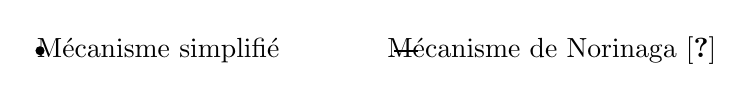
\begin{tikzpicture}
		\draw[fill=black] (0, 0) circle (0.05);
		\node at (1.5, 0) {M\'ecanisme simplifi\'e};
		
		\draw[fill=black, thick] (4.5,0) -- (4.8, 0);
		\node at (6.5, 0) {M\'ecanisme de Norinaga~\cite{Norinaga2009}};
	\end{tikzpicture}
	\vfill{}
	\adjincludegraphics[trim={0 {0.66\height} 0 0},clip,width=14cm]
		{figures/norinaga-comparison-simplification-1173K}
	\vfill{}
\end{frame}


\begin{frame}{\insertsection}{\insertsubsection: \ch{C2H2} -- réacteur piston (BP)}
  \centering{}\footnotesize{}%
  \setlength{\aboverulesep}{0pt}
  \setlength{\belowrulesep}{0pt}
  \setlength{\extrarowheight}{2pt}
     
  \vfill{}
  \only<1>{
    \begin{tabular}{cccccccccccc}
    	\toprule[2pt]
    	\multirow{3}{*}[-3pt]{\bfseries{}N} &
    	\textbf{P} &
    	\textbf{Q} &
    	\textbf{T} &
    	{$\tau_{\mathbf{eff}}$} &
    	{$\delta_{\mathbf{\dot{V}}}$} &
    	\multicolumn{5}{c}{\bfseries{}Fraction molaire en \ch{C2H2}}
    	\tabularnewline
    	\cmidrule{7-12}
    	& 
    	\multirow{2}{*}[+1pt]{\si{\hecto\pascal}}   &
    	\multirow{2}{*}[+1pt]{\si{\sccm}}           & 
    	\multirow{2}{*}[+1pt]{\si{\kelvin}}         & 
    	\multirow{2}{*}[+1pt]{\si{\second}}         &
    	\multirow{2}{*}[+1pt]{\%}                   & 
    	\multicolumn{2}{c}{Mesures}                 &
    	\multicolumn{2}{c}{Norinaga}                &
    	\multicolumn{2}{c}{Simplifié}
    	\tabularnewline
    	\multicolumn{6}{c}{} & Valeur & $F-\%$ & Valeur & $\varepsilon-\%$ & Valeur & $\varepsilon-\%$
    	\tabularnewline
    	\midrule[2pt]
    	%                                                   241            41                             35   
    	1  &  50 & 222 &  773 & 1,836 & 0,0 & 0,352 & 97  & 0,360 & +2,3 & 0,360 & +2,3 \tabularnewline[3pt] % 0,360
    	2  &  50 & 222 &  873 & 1,593 & 0,0 & 0,364 & 100 & 0,359 & -1,4 & 0,360 & -1,1 \tabularnewline[3pt] % 0,359
    	3  &  50 & 222 &  973 & 1,417 & 0,2 & 0,364 & 100 & 0,356 & -2,2 & 0,356 & -2,2 \tabularnewline[3pt] % 0,355
    	4  &  50 & 222 & 1073 & 1,278 & 0,8 & 0,346 & 95  & 0,340 & -1,7 & 0,340 & -1,7 \tabularnewline[3pt] % 0,339
    	5  &  50 & 222 & 1123 & 1,236 & 1,5 & 0,312 & 86  & 0,321 & +2,9 & 0,321 & +2,9 \tabularnewline[3pt] % 0,319
    	6  &  50 & 222 & 1173 & 1,197 & 2,2 & 0,307 & 84  & 0,302 & -1,6 & 0,301 & -2,0 \tabularnewline[3pt] % 0,295
    	7  &  50 & 222 & 1273 & 1,140 & 1,6 & 0,288 & 79  & 0,287 & -0,3 & 0,288 & -0,0 \tabularnewline[3pt] % 0,286
    	8  &  30 & 222 & 1173 & 0,713 & 0,9 & 0,323 & 89  & 0,327 & +1,2 & 0,327 & +1,2 \tabularnewline[3pt] % 0,323
    	9  &  30 & 222 & 1223 & 0,696 & 1,0 & 0,314 & 86  & 0,320 & +1,9 & 0,319 & +1,6 \tabularnewline[3pt] % 0,324
    	10 & 100 & 222 & 1173 & 2,443 & 6,3 & 0,249 & 68  & 0,230 & -7,6 & 0,232 & -6,8 \tabularnewline[3pt] % 0,235
    	11 & 100 & 222 & 1223 & 2,363 & 6,0 & 0,226 & 62  & 0,219 & -3,1 & 0,221 & -2,2 \tabularnewline[3pt] % 0,231
    	12 & 100 & 222 & 1273 & 2,294 & 4,9 & 0,201 & 55  & 0,208 & +3,5 & 0,212 & +5,5 \tabularnewline[3pt] % 0,222
    	13 & 100 & 378 & 1023 & 1,556 & 0,9 & 0,343 & 94  & 0,342 & -0,3 & 0,342 & -0,3 \tabularnewline[3pt] % 0,340
    	14 & 100 & 378 & 1123 & 1,443 & 3,2 & 0,298 & 82  & 0,292 & -2,0 & 0,288 & -3,4
    	\tabularnewline
    	\bottomrule
    \end{tabular}
  }
  \only<2>{
    \newcolumntype{g}{>{\columncolor{red!30}}c}
    
    \begin{tabular}{cccccccccgcg}
    	\toprule[2pt]
    	\multirow{3}{*}[-3pt]{\bfseries{}N} &
    	\textbf{P} &
    	\textbf{Q} &
    	\textbf{T} &
    	{$\tau_{\mathbf{eff}}$} &
    	{$\delta_{\mathbf{\dot{V}}}$} &
    	\multicolumn{5}{c}{\bfseries{}Fraction molaire en \ch{C2H2}}
    	\tabularnewline
    	\cmidrule{7-12}
    	& 
    	\multirow{2}{*}[+1pt]{\si{\hecto\pascal}}   &
    	\multirow{2}{*}[+1pt]{\si{\sccm}}           & 
    	\multirow{2}{*}[+1pt]{\si{\kelvin}}         & 
    	\multirow{2}{*}[+1pt]{\si{\second}}         &
    	\multirow{2}{*}[+1pt]{\%}                   & 
    	\multicolumn{2}{c}{Mesures}                 &
    	\multicolumn{2}{c}{Norinaga}                &
    	\multicolumn{2}{c}{Simplifié}
    	\tabularnewline
    	\multicolumn{6}{c}{} & Valeur & $F-\%$ & Valeur & $\varepsilon-\%$ & Valeur & $\varepsilon-\%$
    	\tabularnewline
    	\midrule[2pt]
    	%                                                   241            41                             35   
    	1  &  50 & 222 &  773 & 1,836 & 0,0 & 0,352 & 97  & 0,360 & +2,3 & 0,360 & +2,3 \tabularnewline[3pt] % 0,360
    	2  &  50 & 222 &  873 & 1,593 & 0,0 & 0,364 & 100 & 0,359 & -1,4 & 0,360 & -1,1 \tabularnewline[3pt] % 0,359
    	3  &  50 & 222 &  973 & 1,417 & 0,2 & 0,364 & 100 & 0,356 & -2,2 & 0,356 & -2,2 \tabularnewline[3pt] % 0,355
    	4  &  50 & 222 & 1073 & 1,278 & 0,8 & 0,346 & 95  & 0,340 & -1,7 & 0,340 & -1,7 \tabularnewline[3pt] % 0,339
    	5  &  50 & 222 & 1123 & 1,236 & 1,5 & 0,312 & 86  & 0,321 & +2,9 & 0,321 & +2,9 \tabularnewline[3pt] % 0,319
    	6  &  50 & 222 & 1173 & 1,197 & 2,2 & 0,307 & 84  & 0,302 & -1,6 & 0,301 & -2,0 \tabularnewline[3pt] % 0,295
    	7  &  50 & 222 & 1273 & 1,140 & 1,6 & 0,288 & 79  & 0,287 & -0,3 & 0,288 & -0,0 \tabularnewline[3pt] % 0,286
    	8  &  30 & 222 & 1173 & 0,713 & 0,9 & 0,323 & 89  & 0,327 & +1,2 & 0,327 & +1,2 \tabularnewline[3pt] % 0,323
    	9  &  30 & 222 & 1223 & 0,696 & 1,0 & 0,314 & 86  & 0,320 & +1,9 & 0,319 & +1,6 \tabularnewline[3pt] % 0,324
    	10 & 100 & 222 & 1173 & 2,443 & 6,3 & 0,249 & 68  & 0,230 & -7,6 & 0,232 & -6,8 \tabularnewline[3pt] % 0,235
    	11 & 100 & 222 & 1223 & 2,363 & 6,0 & 0,226 & 62  & 0,219 & -3,1 & 0,221 & -2,2 \tabularnewline[3pt] % 0,231
    	12 & 100 & 222 & 1273 & 2,294 & 4,9 & 0,201 & 55  & 0,208 & +3,5 & 0,212 & +5,5 \tabularnewline[3pt] % 0,222
    	13 & 100 & 378 & 1023 & 1,556 & 0,9 & 0,343 & 94  & 0,342 & -0,3 & 0,342 & -0,3 \tabularnewline[3pt] % 0,340
    	14 & 100 & 378 & 1123 & 1,443 & 3,2 & 0,298 & 82  & 0,292 & -2,0 & 0,288 & -3,4
    	\tabularnewline
    	\bottomrule
    \end{tabular}
  }
  
  \vfill{}
\end{frame}


\begin{frame}{\insertsection}{\insertsubsection: \ch{NH3} -- réacteur piston (BP)}
  \setlength{\aboverulesep}{0pt}
  \setlength{\belowrulesep}{0pt}
  \setlength{\extrarowheight}{2pt}
  
	\begin{center}\footnotesize{}%
	\only<1>{
  	\begin{tabular}{cccccccccc}
  		\toprule[2pt]
  		\multirow{2}{*}[-3pt]{\bfseries{}N}        &
  		\textbf{Dilution}               &
  		\textbf{P}                      &
  		\textbf{Q}                      &
  		\textbf{T}                      &
  		{$\tau_{\mathbf{eff}}$}         &
  		{$S_{c}$}                       &
  		\multicolumn{3}{c}{\bfseries Fraction molaire en \ch{NH3}}
  		\tabularnewline
  		\cmidrule{8-10} 
  		&                           
  		{x(\ch{NH3})}               &  
  		{\si{\hecto\pascal}}        &
  		{\si{\sccm}}                & 
  		{\si{\kelvin}}              & 
  		{\si{\second}}              &
  		{\si{\square\centi\metre}}  & 
  		{Mesures}                   &
  		{Homogène}                  &
  		{Hétérogène}
  		\tabularnewline
  		\midrule[2pt]
  		1 & 0,25 &  50 & 684 & 1173 & 0,396 & 0,0 & 0,250 & 0,250 & 0,244
  		\tabularnewline[3pt]
  		2 & 0,64 &  50 & 737 & 1173 & 0,369 & 0,0 & 0,640 & 0,640 & 0,622
  		\tabularnewline[3pt]
  		3 & 0,98 &  50 & 470 & 1073 & 0,613 & 0,0 & 0,951 & 0,980 & 0,965
  		\tabularnewline[3pt]
  		4 & 0,98 &  50 & 470 & 1173 & 0,571 & 0,0 & 0,920 & 0,979 & 0,925
  		\tabularnewline[3pt]
  		5 & 0,98 & 100 & 470 & 1073 & 1,248 & 0,0 & 0,927 & 0,979 & 0,950
  		\tabularnewline[3pt]
  		6 & 0,98 & 100 & 470 & 1173 & 1,151 & 0,0 & 0,875 & 0,938 & 0,875
  		\tabularnewline[3pt]
  		7 & 0,23 & 100 & 687 & 1173 & - & 8,80 & 0,193 & - & -
  		\tabularnewline[3pt]
  		8 & 0,64 & 100 & 737 & 1173 & - & 9,54 & 0,413 & - & -
  		\tabularnewline[3pt]
  		9 & 0,64 & 100 & 737 & 1173 & - & 18,1 & 0,391 & - & -
  		\tabularnewline
  		\bottomrule    
  	\end{tabular}	
	}
	\only<2>{
		\newcolumntype{g}{>{\columncolor{red!30}}c}
		
  	\begin{tabular}{cccccccgcg}
  		\toprule[2pt]
  		\multirow{2}{*}[-3pt]{\bfseries{}N}        &
  		\textbf{Dilution}               &
  		\textbf{P}                      &
  		\textbf{Q}                      &
  		\textbf{T}                      &
  		{$\tau_{\mathbf{eff}}$}         &
  		{$S_{c}$}                       &
  		\multicolumn{3}{c}{\bfseries Fraction molaire en \ch{NH3}}
  		\tabularnewline
  		\cmidrule{8-10} 
  		&                           
  		{x(\ch{NH3})}               &  
  		{\si{\hecto\pascal}}        &
  		{\si{\sccm}}                & 
  		{\si{\kelvin}}              & 
  		{\si{\second}}              &
  		{\si{\square\centi\metre}}  & 
  		{Mesures}                   &
  		{Homogène}                  &
  		{Hétérogène}
  		\tabularnewline
  		\midrule[2pt]
  		1 & 0,25 &  50 & 684 & 1173 & 0,396 & 0,0 & 0,250 & 0,250 & 0,244
  		\tabularnewline[3pt]
  		2 & 0,64 &  50 & 737 & 1173 & 0,369 & 0,0 & 0,640 & 0,640 & 0,622
  		\tabularnewline[3pt]
  		3 & 0,98 &  50 & 470 & 1073 & 0,613 & 0,0 & 0,951 & 0,980 & 0,965
  		\tabularnewline[3pt]
  		4 & 0,98 &  50 & 470 & 1173 & 0,571 & 0,0 & 0,920 & 0,979 & 0,925
  		\tabularnewline[3pt]
  		5 & 0,98 & 100 & 470 & 1073 & 1,248 & 0,0 & 0,927 & 0,979 & 0,950
  		\tabularnewline[3pt]
  		6 & 0,98 & 100 & 470 & 1173 & 1,151 & 0,0 & 0,875 & 0,938 & 0,875
  		\tabularnewline[3pt]
  		7 & 0,23 & 100 & 687 & 1173 & - & 8,80 & 0,193 & - & -
  		\tabularnewline[3pt]
  		8 & 0,64 & 100 & 737 & 1173 & - & 9,54 & 0,413 & - & -
  		\tabularnewline[3pt]
  		9 & 0,64 & 100 & 737 & 1173 & - & 18,1 & 0,391 & - & -
  		\tabularnewline
  		\bottomrule    
  	\end{tabular}
  }
	\end{center}
	\vfill{}
	
	Taux de décomposition de l'ammoniac sur des sites de surface du quartz:
	
	$$
	  \ch{NH3 + Q_z -> Produits}\qquad{}
	  \rightarrow{}\qquad{}k{}={}2,71{}\times{}10^{14}{}\exp\biggr(\frac{149\si{\kilo\joule\per\mole}}{RT}\biggr)
	  \quad\si{\per\second}
	$$	
\end{frame}


\section{Conclusions}


\begin{frame}{\insertsection}{Conclusions de l'étude}
  \setbeamercolor{normal text}{fg=gray,bg=}
  \setbeamercolor{alerted text}{fg=black,bg=}
  \usebeamercolor{normal text}
  
  \begin{itemize}
		\item \alert<1->{Simulation vs. expériences: bon accord entre profils mesur\'es et calcul\'es pour la nuance 23MnCrMo5 (maitrise des conditions aux limites); cela n'est pas le cas de la nitruration de la nuance 16NiCrMo13 (r\^ole du nickel).}
		\vfill{}
		
		\item \alert<2->{Nitrures à haute température: la précipitation de \ch{CrN} sur la nuance 16NiCrMo13 a été prédite correctement (confirmé par MET et analyse d'images); la nuance 23MnCrMo5 a conduit à la formation de \ch{MnSiN2}, nitrure absent dans les bases thermodynamiques à notre disposition.}
		\vfill{}
		
		\item \alert<3->{Dureté après trempe: similaire pour la cémentation et la carbonitruration de la nuance 23MnCrMo5; la tenue en dureté après revenu est plus importante pour des échantillons carbonitrur\'es (composite).}
		\vfill{}
		
		\item \alert<4->{Durcissement secondaire mis en évidence après le revenu des aciers nitrurés en phase austénitique, spécialement pour l'alliage 16NiCrMo13. Des études par MET et diffraction d'électrons montrent la présence de nano-précipités de structure \ch{Fe16N2}.}
		\vfill{}
		
		\item \alert<5->{Le comportement global de la pyrolyse d'acétylène décrit dans la littérature a été reproduit et simulé; ces résultats ont servi comme base pour l'obtention d'un mécanisme détaillé plus simple pour des applications industrielles.}
  \end{itemize}
\end{frame}
%
\begin{frame}{\insertsection}{Projections futures}

  \begin{itemize}
		\item Étude par MET de la formation de nano-précipités dans des alliages modèles \ch{Fe - $x$ Cr - N} avec différentes teneurs en chrome et évaluation de son effet sur la tenue en dureté après revenu.
		\vfill{}
		
		\item Analyse par AP-FIM~$^\text{1}$ de la localisation de l'azote \textendash{} comme cela a été réalisé pour le carbone par \citet{Hutchinson20115845} \textendash{} après trempe pour confirmer la validité de l'extension à l'azote du modèle de \citet{Norstrom1976}.
		\vfill{}
		
		\item Étude de la décomposition de l'ammoniac en couplant FTIR et chromatographie gazeuse en présence d'échantillons de différents matériaux métalliques et avec un condensateur à la sortie pour la quantification éventuelle des produits minoritaires.
		\vfill{}
		
		\item Simulation et validation expérimentales à l'échelle semi--industrielle de la décomposition de \ch{C2H2} avec le mécanisme cinétique simplifié obtenu. Ces études doivent incorporer différents chargements et mesures de débits en entrée et en sortie de réacteur.
  \end{itemize}
  \footnotetext[1]{De l'Anglais Atom-probe field-ion microscopy.}
\end{frame}


\begin{frame}
  \vspace{2cm}\Huge\centering{Merci de votre attention!}
\end{frame}


\section{Références}


\begin{frame}[allowframebreaks]{\insertsection}
  \tiny{}\bibliography{references}
\end{frame}


\end{document}


\endinput